\documentclass{article}
\begin{document}
\section{INFO1903 Project}\label{info1903-project}

\subsection{Section I: Data analysis}\label{section-i-data-analysis}

\subsubsection{Situation \{\#situation\}}\label{situation-situation}

For this project, I wanted to analyse state rainfall data\\
alongside road fatalities, with the primary aim of finding\\
a correlation between the two.

\subsubsection{Data Sources \{\#sources\}}\label{data-sources-sources}

\paragraph{Online Sources}\label{online-sources}

\begin{itemize}
\tightlist
\item
  \href{http://data.gov.au/dataset/australian-road-deaths-database/resource/ca07c8e3-672f-4826-a6e5-83fd7127ae0b}{The
  Australian Road Deaths Database}) which contains information about the
  crashes and the fatalities.
\item
  \href{http://www.bom.gov.au/jsp/ncc/cdio/weatherData/av?p_nccObsCode=136\&p_display_type=dailyDataFile\&p_startYear=\&p_c=\&p_stn_num=086039}{The
  Bureau of Meteorology's Daily Rainfall Data} for the station of
  Flemington in Victoria.
\end{itemize}

\paragraph{Download Links:
\{\#downloads\}}\label{download-links-downloads}

\begin{itemize}
\tightlist
\item
  \href{https://bitre.gov.au/statistics/safety/files/Fatal_Crashes_Feb2017.csv}{Crash
  database} (csv)
\item
  \href{https://bitre.gov.au/statistics/safety/files/ARDD_Dictionary_V3.pdf}{Crash
  database legend} (pdf)
\item
  \href{http://www.bom.gov.au/jsp/ncc/cdio/weatherData/av?p_display_type=dailyZippedDataFile\&p_stn_num=086039\&p_c=-1480557288\&p_nccObsCode=136\&p_startYear=2017}{Rain
  database} (csv)
\end{itemize}

\subsubsection{Graphs \{\#graphs\}}\label{graphs-graphs}

After setting up the data, I first graphed the rainfall over time and
the crashes over time to see if I could spot any trends among the
separate graphs:

\paragraph{Car Crashes per Month}\label{car-crashes-per-month}

\href{assets/crashes_over_time.png}{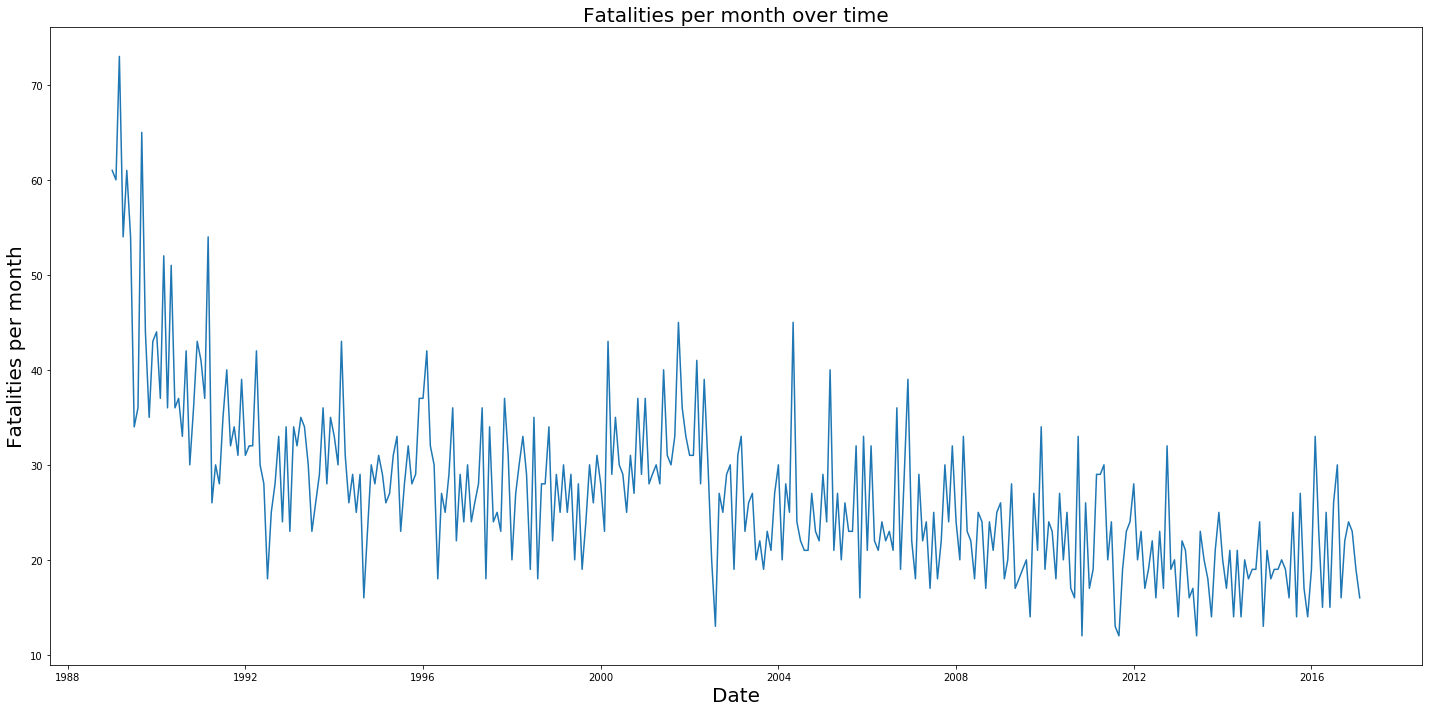
\includegraphics{assets/crashes_over_time.png}}

\begin{center}\rule{0.5\linewidth}{\linethickness}\end{center}

\paragraph{Monthly Rainfall}\label{monthly-rainfall}

\href{assets/rainfall_over_time.png}{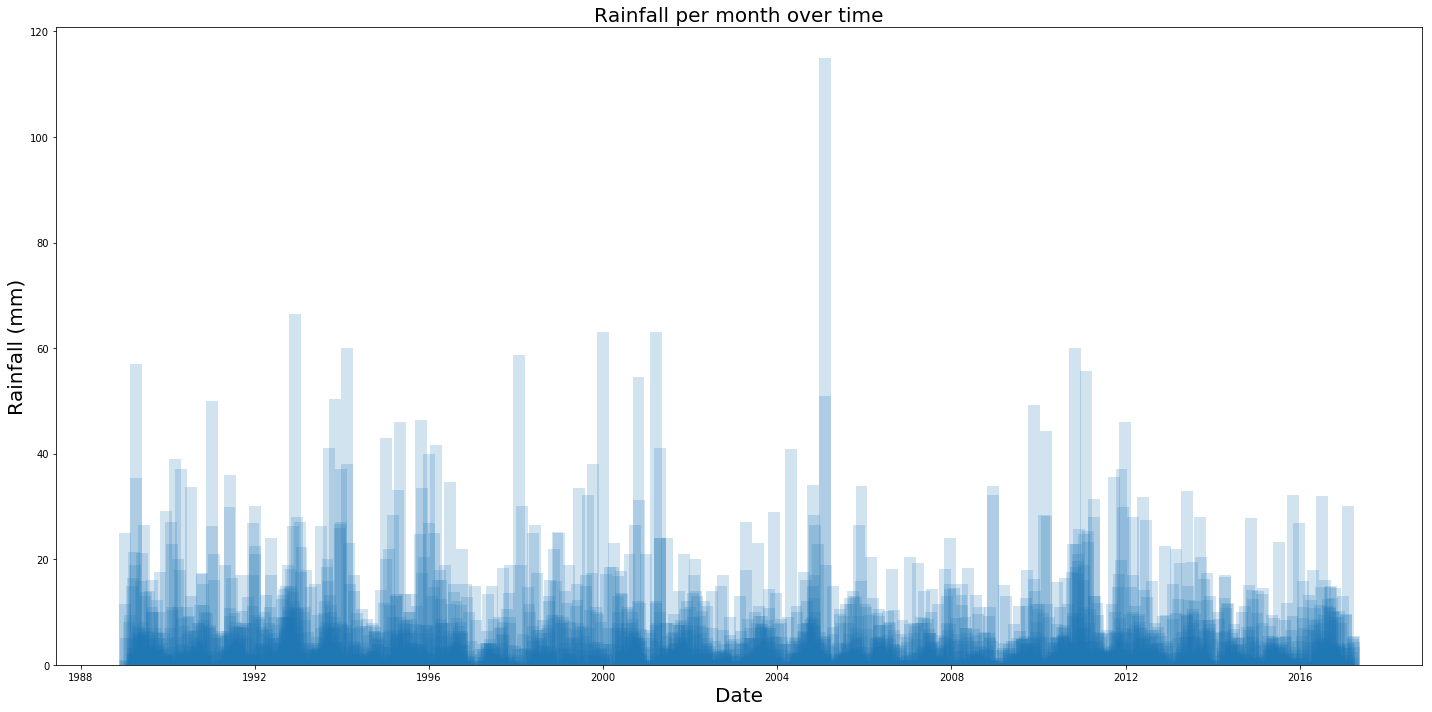
\includegraphics{assets/rainfall_over_time.png}}

\begin{center}\rule{0.5\linewidth}{\linethickness}\end{center}

\paragraph{Crashes and Rainfall over
Time}\label{crashes-and-rainfall-over-time}

After having graphed the data separately, I graphed them on top of each
other to get a better idea at a correlation:

\href{assets/rainfall_vs_deaths.png}{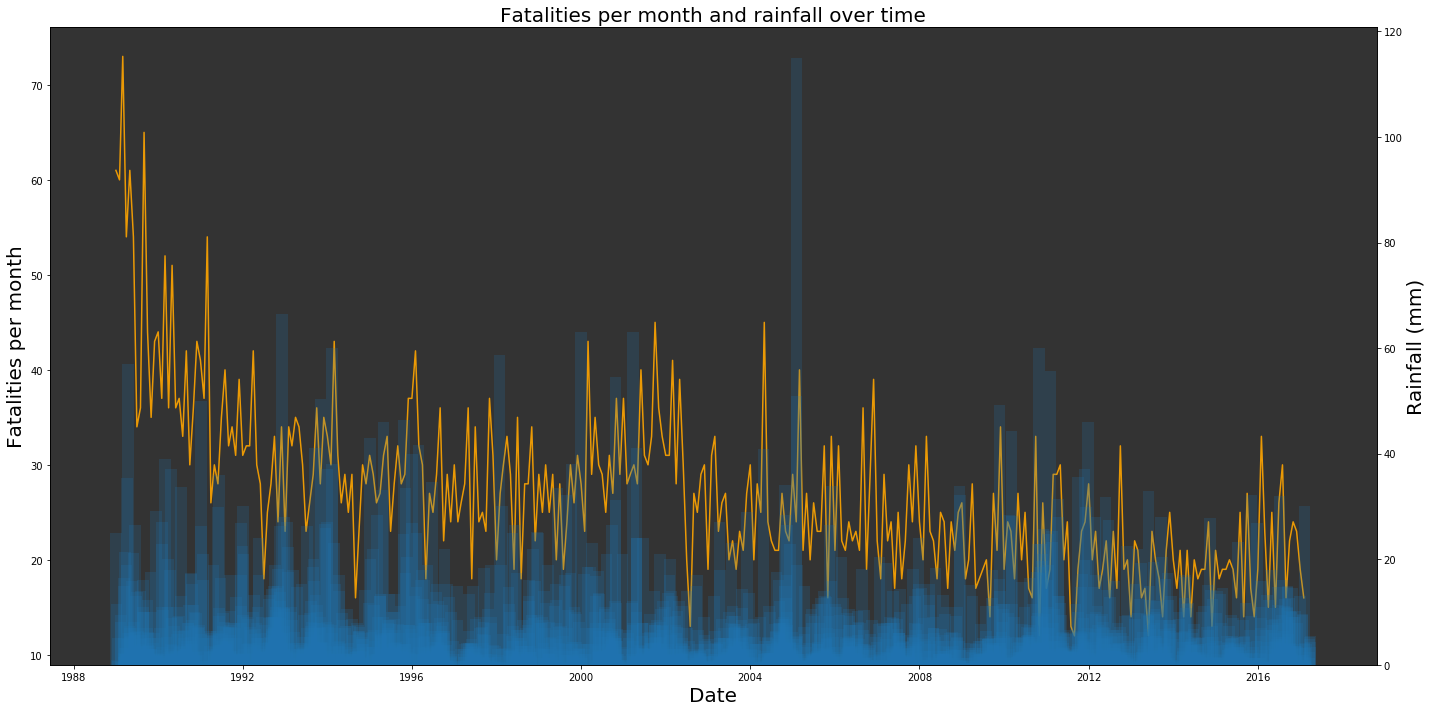
\includegraphics{assets/rainfall_vs_deaths.png}}

\begin{center}\rule{0.5\linewidth}{\linethickness}\end{center}

This final graph is the same data but in a different style: the data
points are the\\
fatalities per month, but the rainfall is instead represented as the
colour of the points.

I thought that this would help visualise the correlation, but it doesn't
really work.

\href{assets/fatalities_vs_date.png}{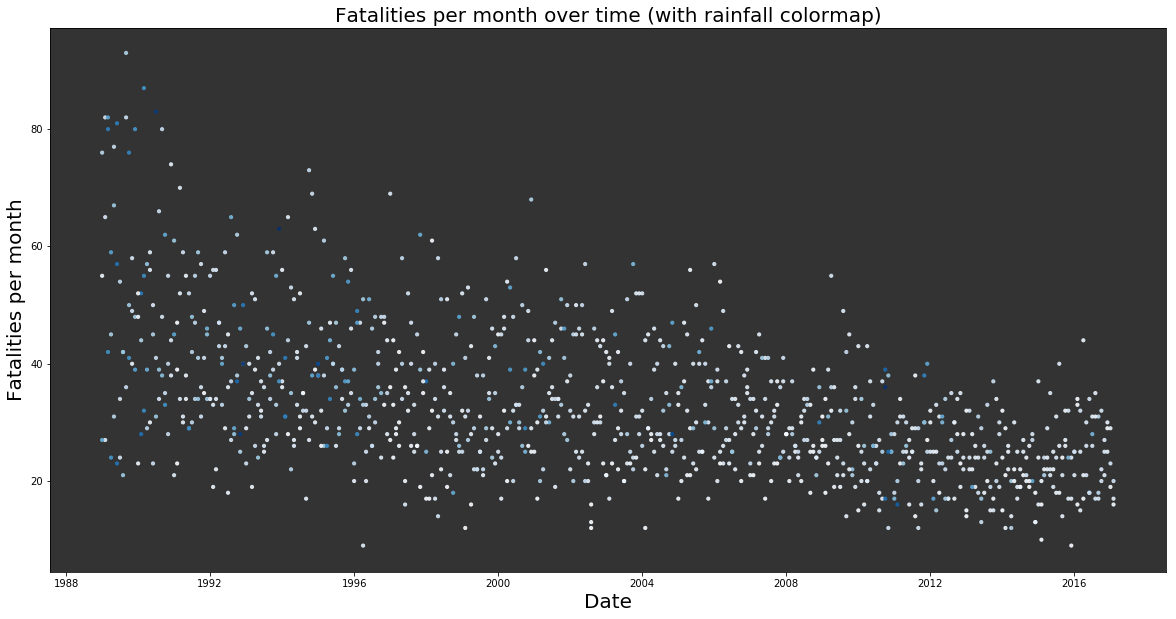
\includegraphics{assets/fatalities_vs_date.png}}

\subsubsection{Discussion \{\#discussion\}}\label{discussion-discussion}

\paragraph{Trends \{\#trends\}}\label{trends-trends}

The crashes/time graph shows that the average number of fatal car
crashes per month has\\
decreased since 1989, something which I expected to see.

\href{assets/crashes_over_time_zoom.png}{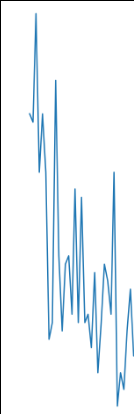
\includegraphics{assets/crashes_over_time_zoom.png}}\\
The spike at the start is because of the Kempsey Bus Crash, cited as the
most\\
deadly road accident in Australia's history.\\
(\href{https://en.wikipedia.org/wiki/Kempsey_bus_crash}{Wikipedia
Article})

\begin{center}\rule{0.5\linewidth}{\linethickness}\end{center}

In the rainfall/time graph, there is an outlier around 2005 - a heavy
rain event.\\
(\href{https://bom.gov.au/climate/annual_sum/2005/page13-15.pdf}{BOM
report})

\paragraph{Results \{\#results\}}\label{results-results}

\paragraph{Further Research
\{\#further-research\}}\label{further-research-further-research}

\subsection{Section II: Data Generation
\{\#generation\}}\label{section-ii-data-generation-generation}

\subsubsection{Getting the data
\{\#obtaining\}}\label{getting-the-data-obtaining}

The website had two datasets available: one for each crash, and one for
each fatality.\\
I chose to use the one per crash, as I was not interested in statistics
such as gender\\
or age. However, the process required to obtain and store this data is
available with the\\
methods for the other files.

\begin{center}\rule{0.5\linewidth}{\linethickness}\end{center}

Due to the nature of the weather, I decided that getting the ``total
national rainfall''\\
was not precise enough. Because the crash data sorted by state (and did
not give a\\
precise location), I decided to pick a state and use only crash data
from that state.

The BOM data provides rainfall data for every weather station back to
the 19th century.\\
As my crash data location had state-level precision, I reasoned that if
I chose a weather\\
station in the middle of a state, it would give me the best approximate
for ``average\\
statewide weather''.

I chose Victoria, as it is a small state with a weather station
(Flemington station)\\
somewhat near both the center of the state and the capital city, where I
reasoned the\\
most crashes would occur.

\subsubsection{Storing in PostgreSQL
\{\#postgres\}}\label{storing-in-postgresql-postgres}

\paragraph{Entering into database}\label{entering-into-database}

\paragraph{Database Schema}\label{database-schema}

\subparagraph{\texorpdfstring{\texttt{crashes}
Table}{crashes Table}}\label{crashes-table}

\begin{longtable}[]{@{}lll@{}}
\toprule
Column & Type & Description\tabularnewline
\midrule
\endhead
\texttt{crashid} & \texttt{character(13)} & Internal crash
ID\tabularnewline
\texttt{state} & \texttt{character\ varying(3)} & State that the crash
occured in\tabularnewline
\texttt{day} & \texttt{integer} & Day of the crash\tabularnewline
\texttt{month} & \texttt{character\ varying(10)} & Month of the crash
(long name format)\tabularnewline
\texttt{year} & \texttt{integer} & Year of the crash\tabularnewline
\texttt{hour} & \texttt{integer} & Hour of the crash\tabularnewline
\texttt{minute} & \texttt{integer} & Minute of the crash\tabularnewline
\texttt{crashtype} & \texttt{character} varying(16) & Internal type of
the crash\tabularnewline
\texttt{fatalities} & \texttt{integer} & Number of
fatalities\tabularnewline
\texttt{bus} & \texttt{boolean} & Was a bus involved?\tabularnewline
\texttt{heavytruck} & \texttt{boolean} & Was a heavy truck
involved?\tabularnewline
\texttt{articulatedtruck} & \texttt{boolean} & Was an articulated truck
involved?\tabularnewline
\texttt{speedlimit} & \texttt{integer} & The speed limit of the
crash\tabularnewline
\bottomrule
\end{longtable}

\subparagraph{\texorpdfstring{\texttt{rainfall}
Table}{rainfall Table}}\label{rainfall-table}

\begin{longtable}[]{@{}lll@{}}
\toprule
Column & Type & Description\tabularnewline
\midrule
\endhead
\texttt{year} & \texttt{integer} & Year of the
measurement\tabularnewline
\texttt{month} & \texttt{integer} & Month of the measurement (in integer
form)\tabularnewline
\texttt{day} & \texttt{integer} & Day of the measurement\tabularnewline
\texttt{rainfall} & \texttt{double\ precision} & Amount of
rainfall\tabularnewline
\texttt{period} & \texttt{integer} & Period measured\tabularnewline
\texttt{quality} & \texttt{character(1)} & Quality of
data\tabularnewline
\bottomrule
\end{longtable}

\paragraph{Issues}\label{issues}

\subparagraph{Date Formatting}\label{date-formatting}

Looking at the above schema, you might notice: the \texttt{month} field
of the rainfall table is\\
an \texttt{integer} type, but \texttt{crashes.month} is a
\texttt{varchar(10)}. \texttt{crashes.month} is a long month\\
name, e.g. \texttt{January}, \texttt{February}.

This was a problem. I had two different formats of data that were needed
to do an\\
SQL JOIN. Luckily, PostgreSQL has a very good set of date formatting
commands.

I decided to leave the tables as they were, and convert the data on the
fly when doing the\\
SQL JOIN. The following SQL functions will convert a date in long format
to an integer:

\begin{verbatim}
extract(MONTH from to_date(concat(crashes.month, ' 2000'), 'Month YYYY'))
\end{verbatim}

\subsubsection{Querying \{\#querying\}}\label{querying-querying}

\paragraph{Issues}\label{issues-1}

\subsubsection{Graphing \{\#graphing\}}\label{graphing-graphing}

\paragraph{Issues}\label{issues-2}

\subsubsection{Notebook \{\#notebook\}}\label{notebook-notebook}

\href{https://nbviewer.jupyter.org/github/lyneca/info1903/blob/gh-pages/INFO1903.ipynb}{Here}\\
is the Jupyter Notebook that contains code for querying and visualising
the data.
\end{document}
